\chapter{Results -- Performance and Analysis}

As stated in the introduction, in the course of this thesis not only platform and agents were implemented, but the agents were also tested in an attempt answer the research questions from section~\ref{sec:researchquestions}. The testing took place on a \keyword{Windows 10 Pro} machine, using GPU-accelerated Tensorflow with an \keyword{NVIDIA GeForce GTX 970} graphics card. In this section, the performance of several agents is visualized and compared to assess their quality. Trends in these plots serve as basis to answer the research questions. 

Unfortunately, the analysis of the implemented agents was restricted a lot by the time limit of this thesis, which also incorporated implementing the platform and writing this text. Also, testing if models and agents while implementing them takes a significant amount of time, as mistakes can be seen only after hours of training. Because also training the agent takes a significant amount of time, the plots given here are the result of much less training episodes than in for example \cite{mnih_human-level_2015}.

If not explicitly mentioned otherwise, all agents use the same hyperparameters, as specified in their respective file\footnote{All agent's path is \url{https://github.com/cstenkamp/BA-rAIce-ANN/tree/master/agents}. The title of the respective file is stated in text and figure.} or in the general config-file\footnote{\url{https://github.com/cstenkamp/BA-rAIce-ANN/blob/master/config.py}}.


\section{General performance}

The general performance of agents can only be assessed in comparison to a baseline. In figures~\ref{fig:humandrive} and figures~\ref{fig:randomdrive}, exemplary laps as driven by a human or a random policy are depicted. In both plots, en episode is either ended by hitting a wall, finishing a round or after 60 seconds time. Note that negative progresses are possible because all agents start at a certain point around $8\%$ in front of the start/finish line. Laptime also advances not until this line is passed.

As can be seen in figure~\ref{fig:randomdrive}, the baseline performance of a random agent is negligible. While it sometimes advances some distance and does not bump into walls for some seconds, it can unmistakenly be seen that the baseline as provided by a random policy is almost zero.

Figure~\ref{fig:humandrive} shows the performance of a human tester with several hours of driving experience for this game. Many of the episodes driven by a human also end with the car hitting the wall, however there are also many episodes in which a full lap was driven. The time taken for an episode by human testers lays between $32$ and $60$ seconds (typically around $32$-$35$ seconds), with no lap driven faster than that.

As can be seen in the progress-plots of the agents (for example in figure~\ref{fig:ddpg_result}), the game appears to have some very obvious local optima. These local optima are at about $16\%$, $40\%$, $60\%$ and $75\%$ and correspond to sharp curves of the track.

Due to severe memory contraints of the provided machine and the fact that agents need a replay memory of hundreds of thousands of states, testing of RL-agents using the minimaps as observation was impossible. However, as the supervised agent that also relied on this observation archived an outstanding accuracy, it is assumed that all findings for the $novision$-agents also hold for their respective counterpart.

The first research question, formalized as \textit{how agents that rely purely on pretraining perform in comparison to reinforcement learning agents}, will be answered in the following section.

\subsection{Supervised agents}

It is hard to assess the performance of purely supervisedly trained agents. Most agents archieved an accuracy of more than $95\%$ on a testing set\footnote{Supervised agents are tested on the \codeobj{.svlap}-files found in \url{https://github.com/cstenkamp/BA-rAIce-ANN/tree/master/SavedLaps}. To generate a testing set, one of the files was removed from the training set.}, but failed completely when tested as agent on the game. The reason for this is easy to see: In this game, one false action at the start can only be fatal, and a supervised agent cannot learn to recover from this mistake.

Testing showed that agents that rely purely on supervised pre-training are not able to drive around the track when tested. Figure~\ref{fig:sv_result} shows this exemplary in the form of an agent that was trained for 75 episodes on a dataset of $27$ exported laps, archieving a testing set accuracy of $93\%$.

\colorbox{red}{dass der hier mit visionvector getestet wurde und das das reicht!!}

\begin{figure}[h]
	{%
		\setlength{\fboxsep}{0pt}%
		\setlength{\fboxrule}{1pt}%
		\fbox{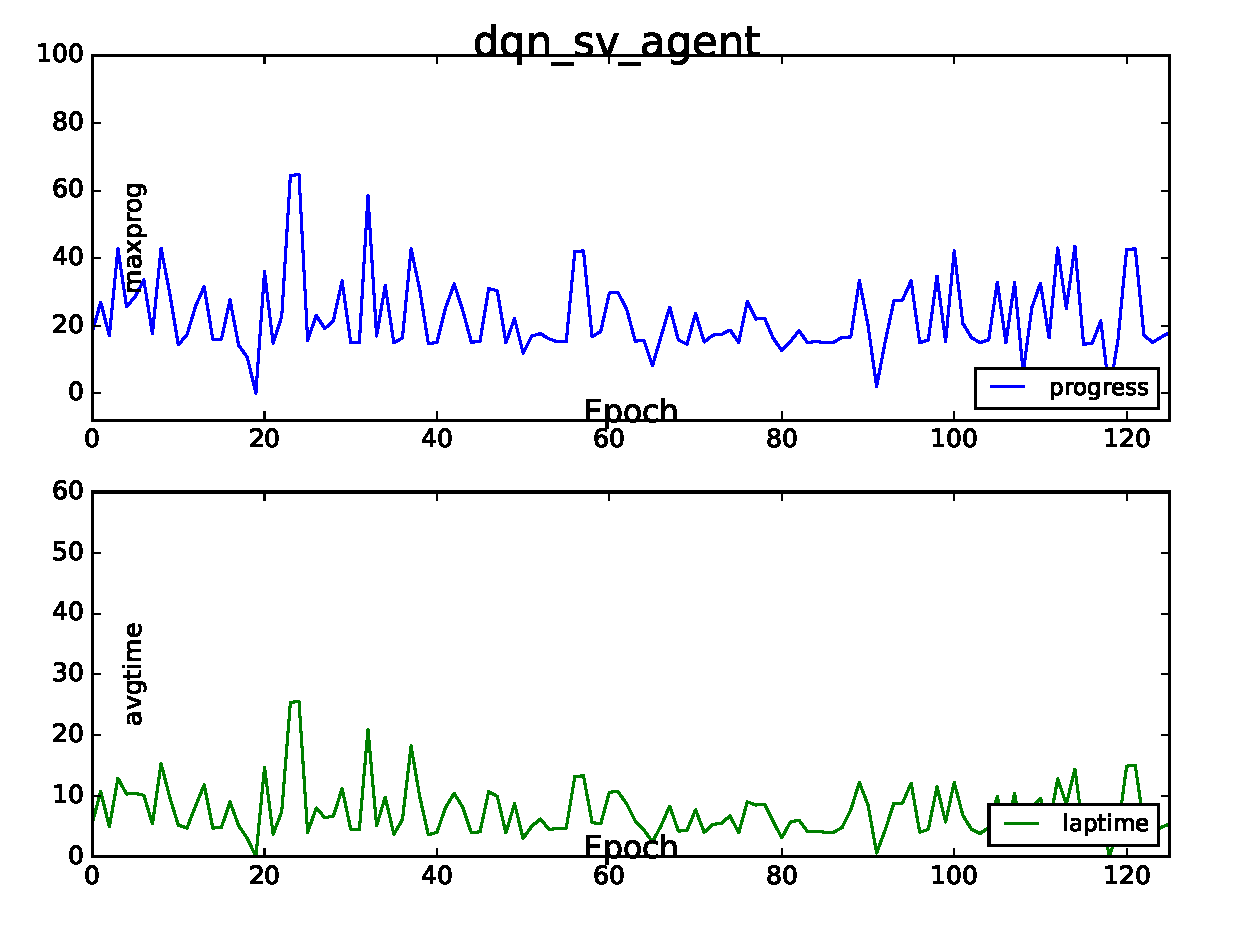
\includegraphics[width=.7\textwidth]{performance_plots/svagent_75pretrains}}%
	}%
	\centering
	\caption[Exemplary performance of the dqn\_sv\_agent]{Exemplary performance of the dqn\_sv\_agent.}
	\label{fig:sv_result}
\end{figure}

As can be seen in this plot, high testing set accuracy does not mean that an agent drives a useful policy. An interesting finding was, that if a maximum-speed of $80$ kph ($33\%$ of \codeobj{Consts.maxSpeed}) was given for both generating the dataset as well as the agent that learns on it, some supervised agents were able to learn successful policies, completing a lap almost every time.

\subsection{RL agents}

The first and foremost result is, that some agents were able to learn successful policies that are able to drive complete laps in a reasonable time. Exemplary performances of the \term{dqn\_novision\_rl\_agent} and the \term{ddpg\_novision\_rl\_agent} are represented in figures \ref{fig:dqn_result} and \ref{fig:ddpg_result}. Note that the training for both agents was terminated as soon as they learned a policy that completes the circuit. Note further, that in all plots that smooth over a specified number of episodes, the maximum reward, Q-value and progress of these episodes is taken.

Testing of the generated Q-values showed that the model that the agents learned has many expected properties, for example 1) the state-value of a state immediately in front of wall is much lower than everywhere else, 2) the q-value of braking is lower than the one of accelerating in a straight street, but higher in close proximities to a turn or wall, 3) steering away from a wall has a higher Q-value than doing nothing or driving towards it, and 4) driving fast leads generally to higher state-values than driving slow. 

It is also very obvious that agents seem to often learn \textit{turn by turn}, in that the track between the sharp turns is always easily made, whereas an agent always seems to need a large number of episodes to overcome a new turn.

\section{Discretizing actions}

This section serves to answer the stated research question of \textit{how different models perform in comparison, and specifically if discretizing the action-space impairs performance}. To do so, the difference between performances of the \term{dqn\_novision\_rl\_agent} and the \term{ddpg\_novision\_rl\_agent} will be elaborated.
Both agents use the same reward function as specified in section~\ref{sec:reward}, as well as the \term{novision}-observation function from section~\ref{sec:observation}. They only differ in their model and, due to that, their exploration-function.

An exemplary performance of the \term{dqn\_novision\_rl\_agent} can be seen in figure~\ref{fig:dqn_result}. The performance of the \term{ddpg\_novision\_rl\_agent} is depicted in figure~\ref{fig:ddpg_result}.

In both cases, the Q-value, average reward and progress increases throughout training. Both agents are further able to complete a whole lap. To do so, DQN-agent required however around 3000 training episodes (over 400.000 minibatch-trainingsteps), whereas the DDPG-agent needed only around 1400 episodes (corresponding to less than 300.000 inferences). It is further interesting, the DQN-agent seems to learn incrementally, where each turn requires hundres of iterations on its own. In contrast to that, the DDPG-agent seems to generalize better from the first part of the track towards the whole track, as can be seen in the very steep learning curve towards the end.

This result shows that while an agent that discretizes the action-space can certainly learn the track, an agent that does so seems to learn slower than its continuous counterpart. As the continuous agent however also used a better exploration function, it is an open question how much of this performance gain must be accredited to that. 

Another question that remains open is, how much faster the laps driven by a continuous agent are will ultimately be. No full lap driven by either of the agents finished in less than $50$ seconds time, which is a lot more than the human average. 

\begin{figure}[h!]
		{%
			\setlength{\fboxsep}{0pt}%
			\setlength{\fboxrule}{1pt}%
			\fbox{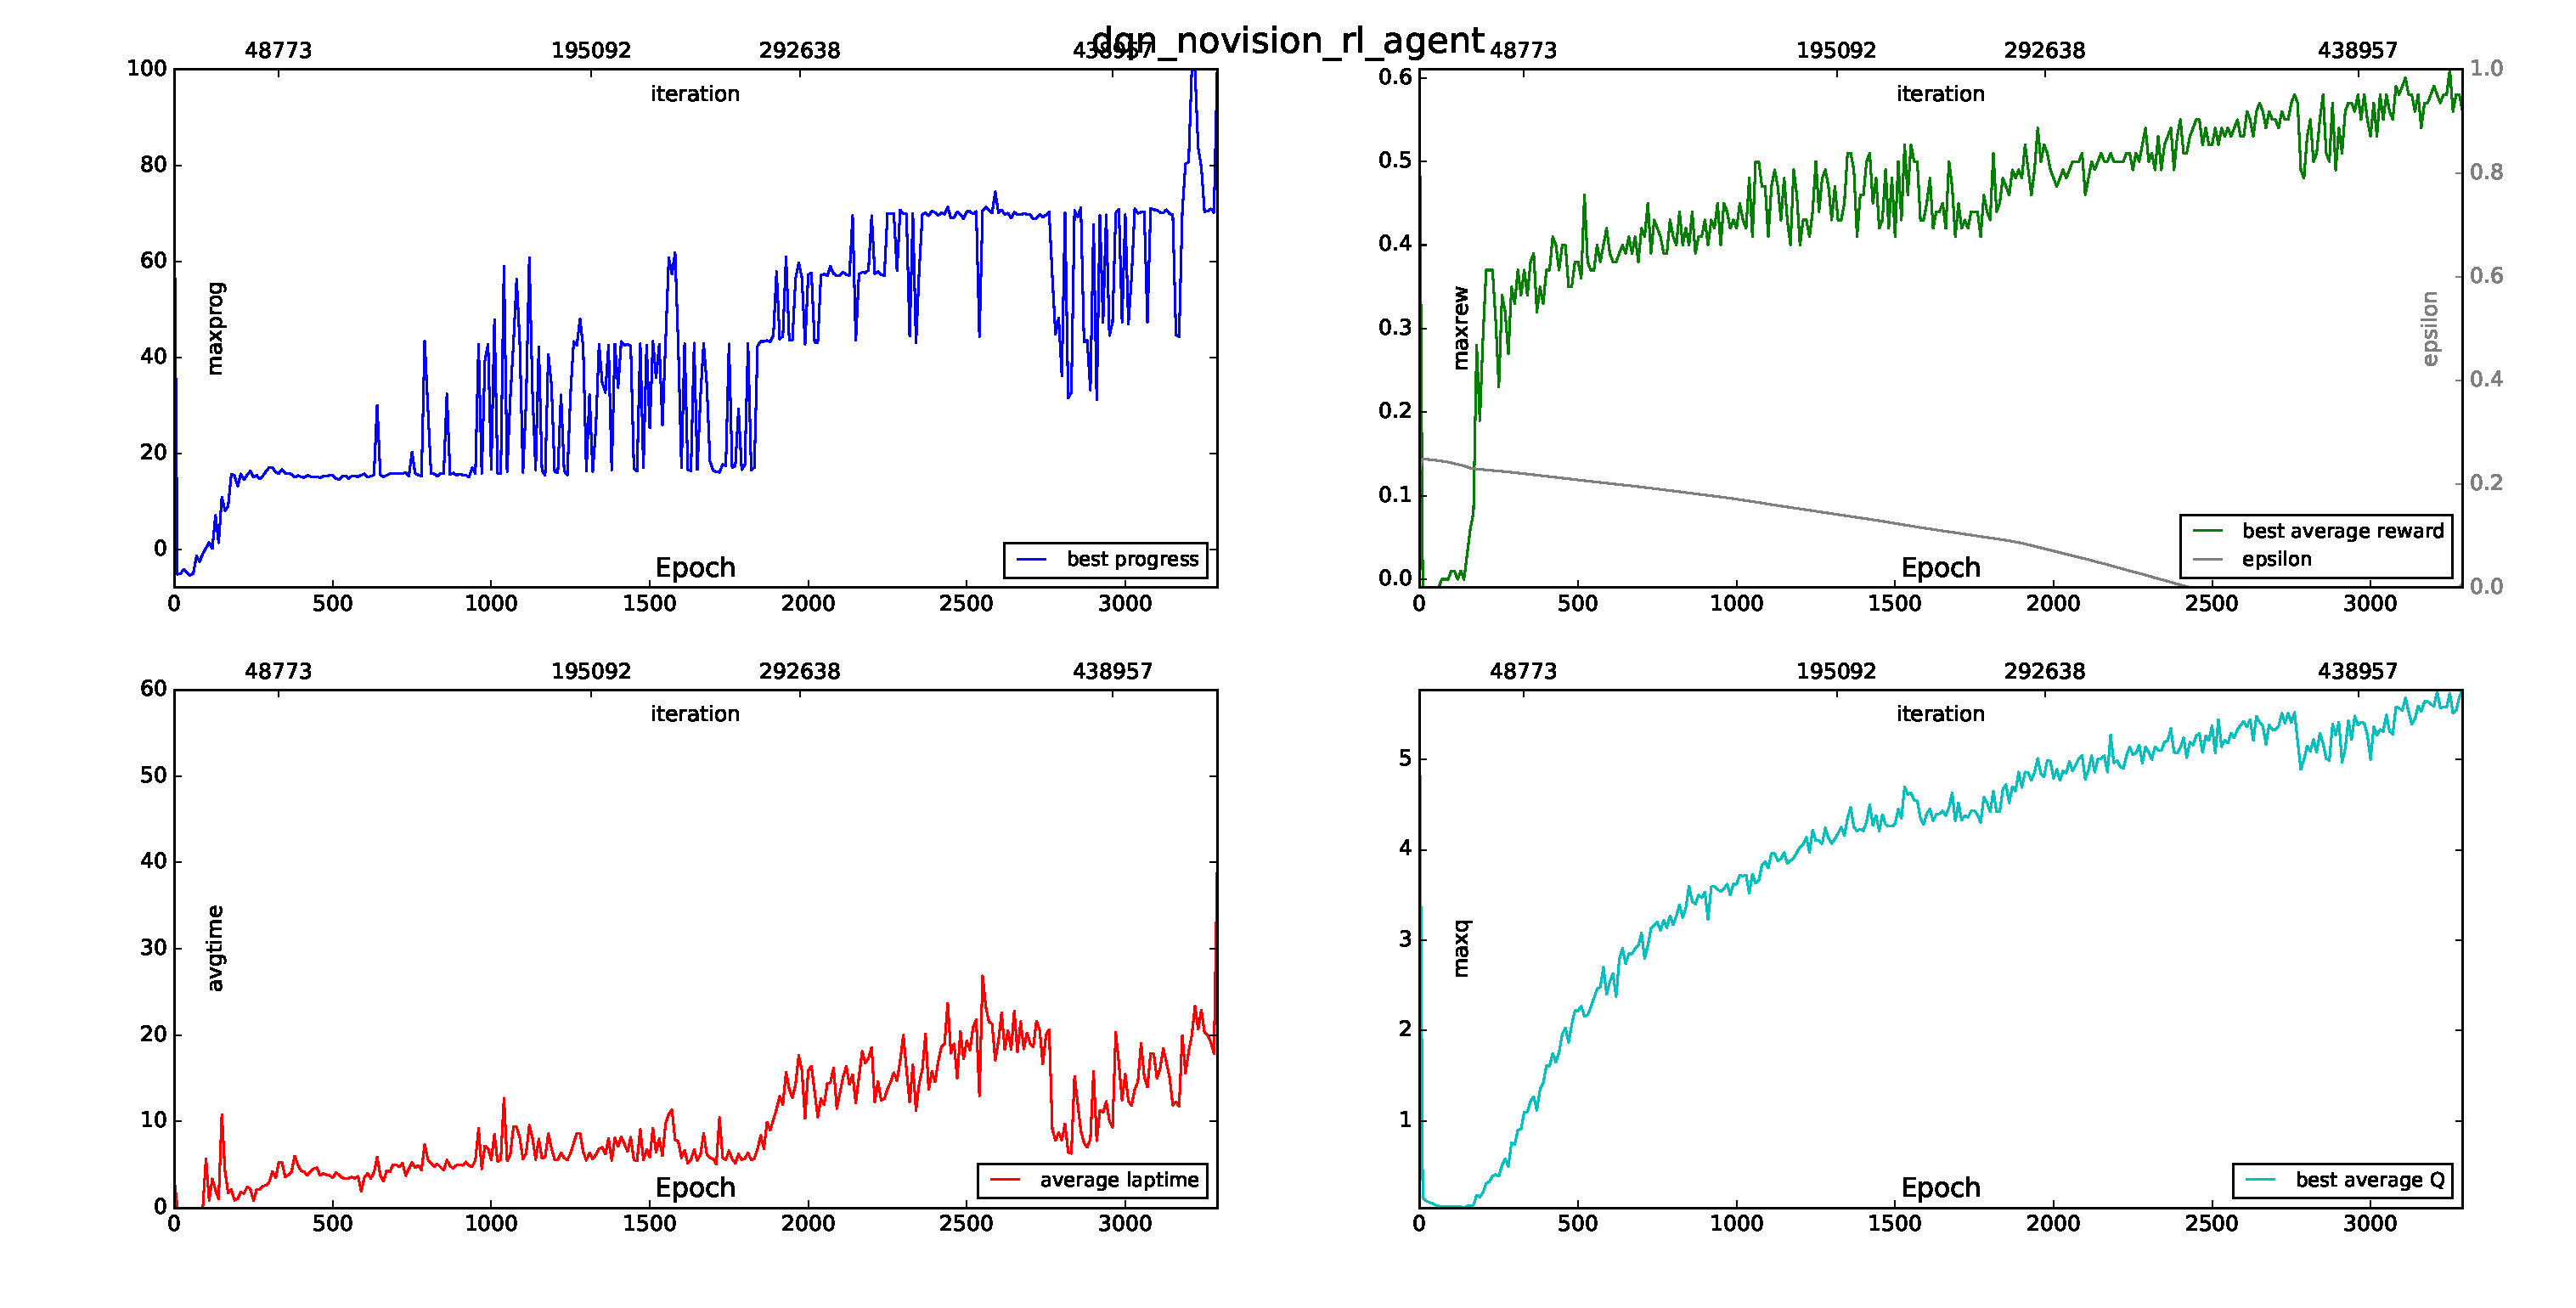
\includegraphics[trim={2.2cm 0cm 1cm 0cm},clip,width=\textwidth]{performance_plots/dqn_bestresult_meinreward_average10_3500ep}}%
		}%
	\centering
	\caption[Exemplary performance of the dqn\_novison\_rl\_agent]{Exemplary performance of the dqn\_novison\_rl\_agent. Plots are smoothed by averaging over 10 episodes.}
	\label{fig:dqn_result}
\end{figure}


\begin{figure}[h!]
{%
	\setlength{\fboxsep}{0pt}%
	\setlength{\fboxrule}{1pt}%
	\fbox{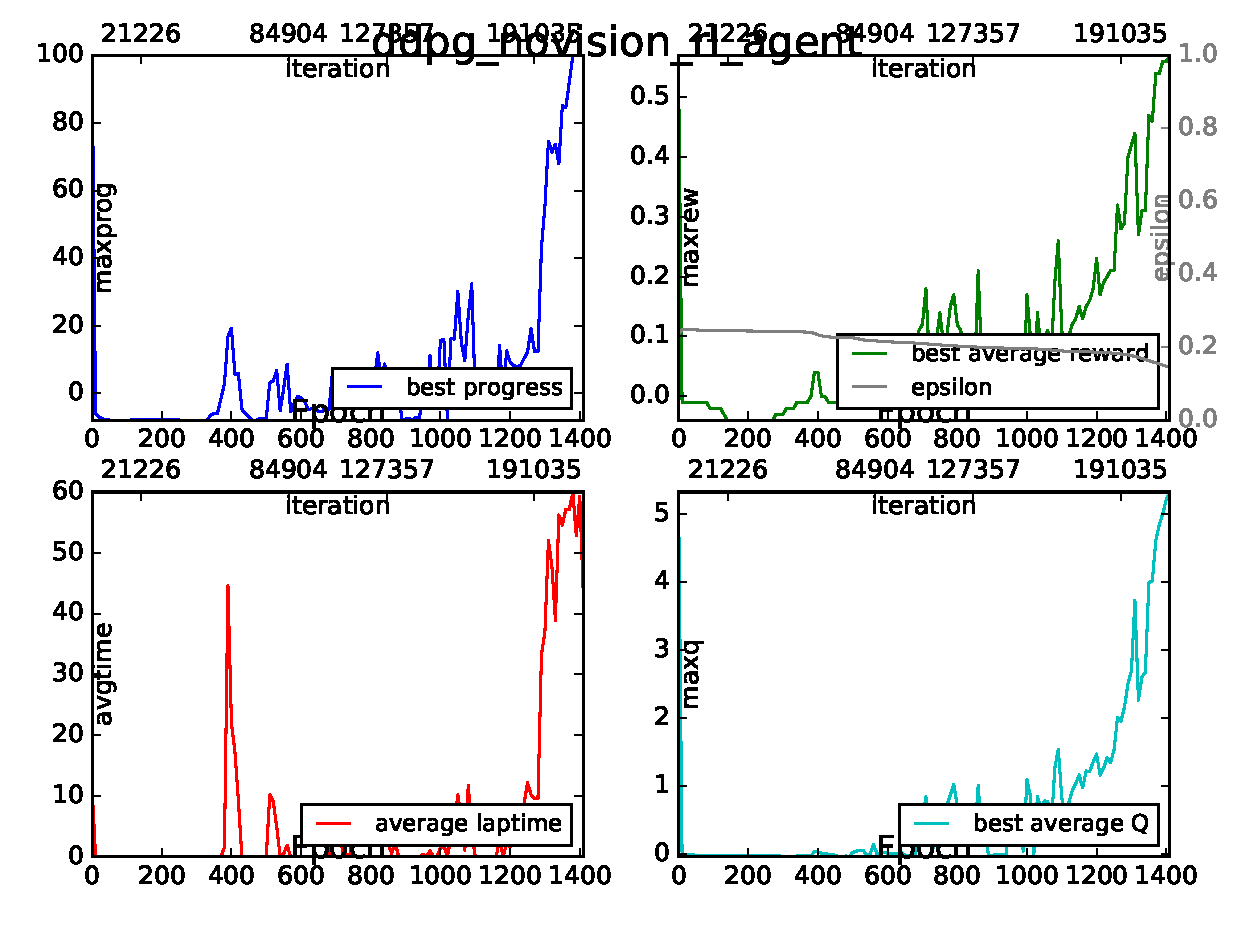
\includegraphics[width=\textwidth]{performance_plots/ddpg_bestresult_meinreward_average10_1400ep}}%
}%
\centering
\caption[Exemplary performance of the ddpg\_novison\_rl\_agent]{Exemplary performance of the ddpg\_novison\_rl\_agent. Plots are smoothed by averaging over 10 episodes.}
\label{fig:ddpg_result}
\end{figure}


\section{Incorporating pretraining}
\label{sec:incorporatePre}

One question this thesis aimed to answer is \textit{how to incorporate pretraining into reinforcedly learning agents}. As explained in section~\ref{sec:pretrainingcode}, an agent that trained supervisedly does not adequatly \keyword{transfer} this knowledge when applied to a reinforcement leaning paradigm. In this thesis, it was tried to find a solution for that by setting correct Q-values for the respective actions, while setting a Q-value of zero for all others.

To test if pretraining an agent increases the learning pace, an agent that performed q-pretraining as specified in section~\ref{sec:pretrainingcode} subsequently underwent normal reinforcement training. Specifically, a \term{ddpg\_novision\_rl\_agent} was pre-trained for $40.000$ pretraining steps on a dataset consisting of $46$ laps (around $14.000$ individual datapoints), such that it had a testing set performance of $96\%$. While the testing set accuracy is high, this agent barely got further than the first turn of the track.

Figure~\ref{fig:ddpg_incorpPre} shows the performance of this agent in actual reinforcement learning. As can be seen, while the rewards and q-values are high at the beginning, it seems impossible for the agent to use that knowledge. In fact, the graph rather suggests the opposite: 1) the reward drops very fast to zero, and stays close to zero for longer time than a non-pretrained agent, 2) the progress-milestone of $16\%$ is reached at around the same time than in an agent that did not perform pretraining (epoch 1300), and 3) The q-value is decreasing until this episode, rising only with the rise of the reward.

\begin{figure}[h]
	{%
		\setlength{\fboxsep}{0pt}%
		\setlength{\fboxrule}{1pt}%
		\fbox{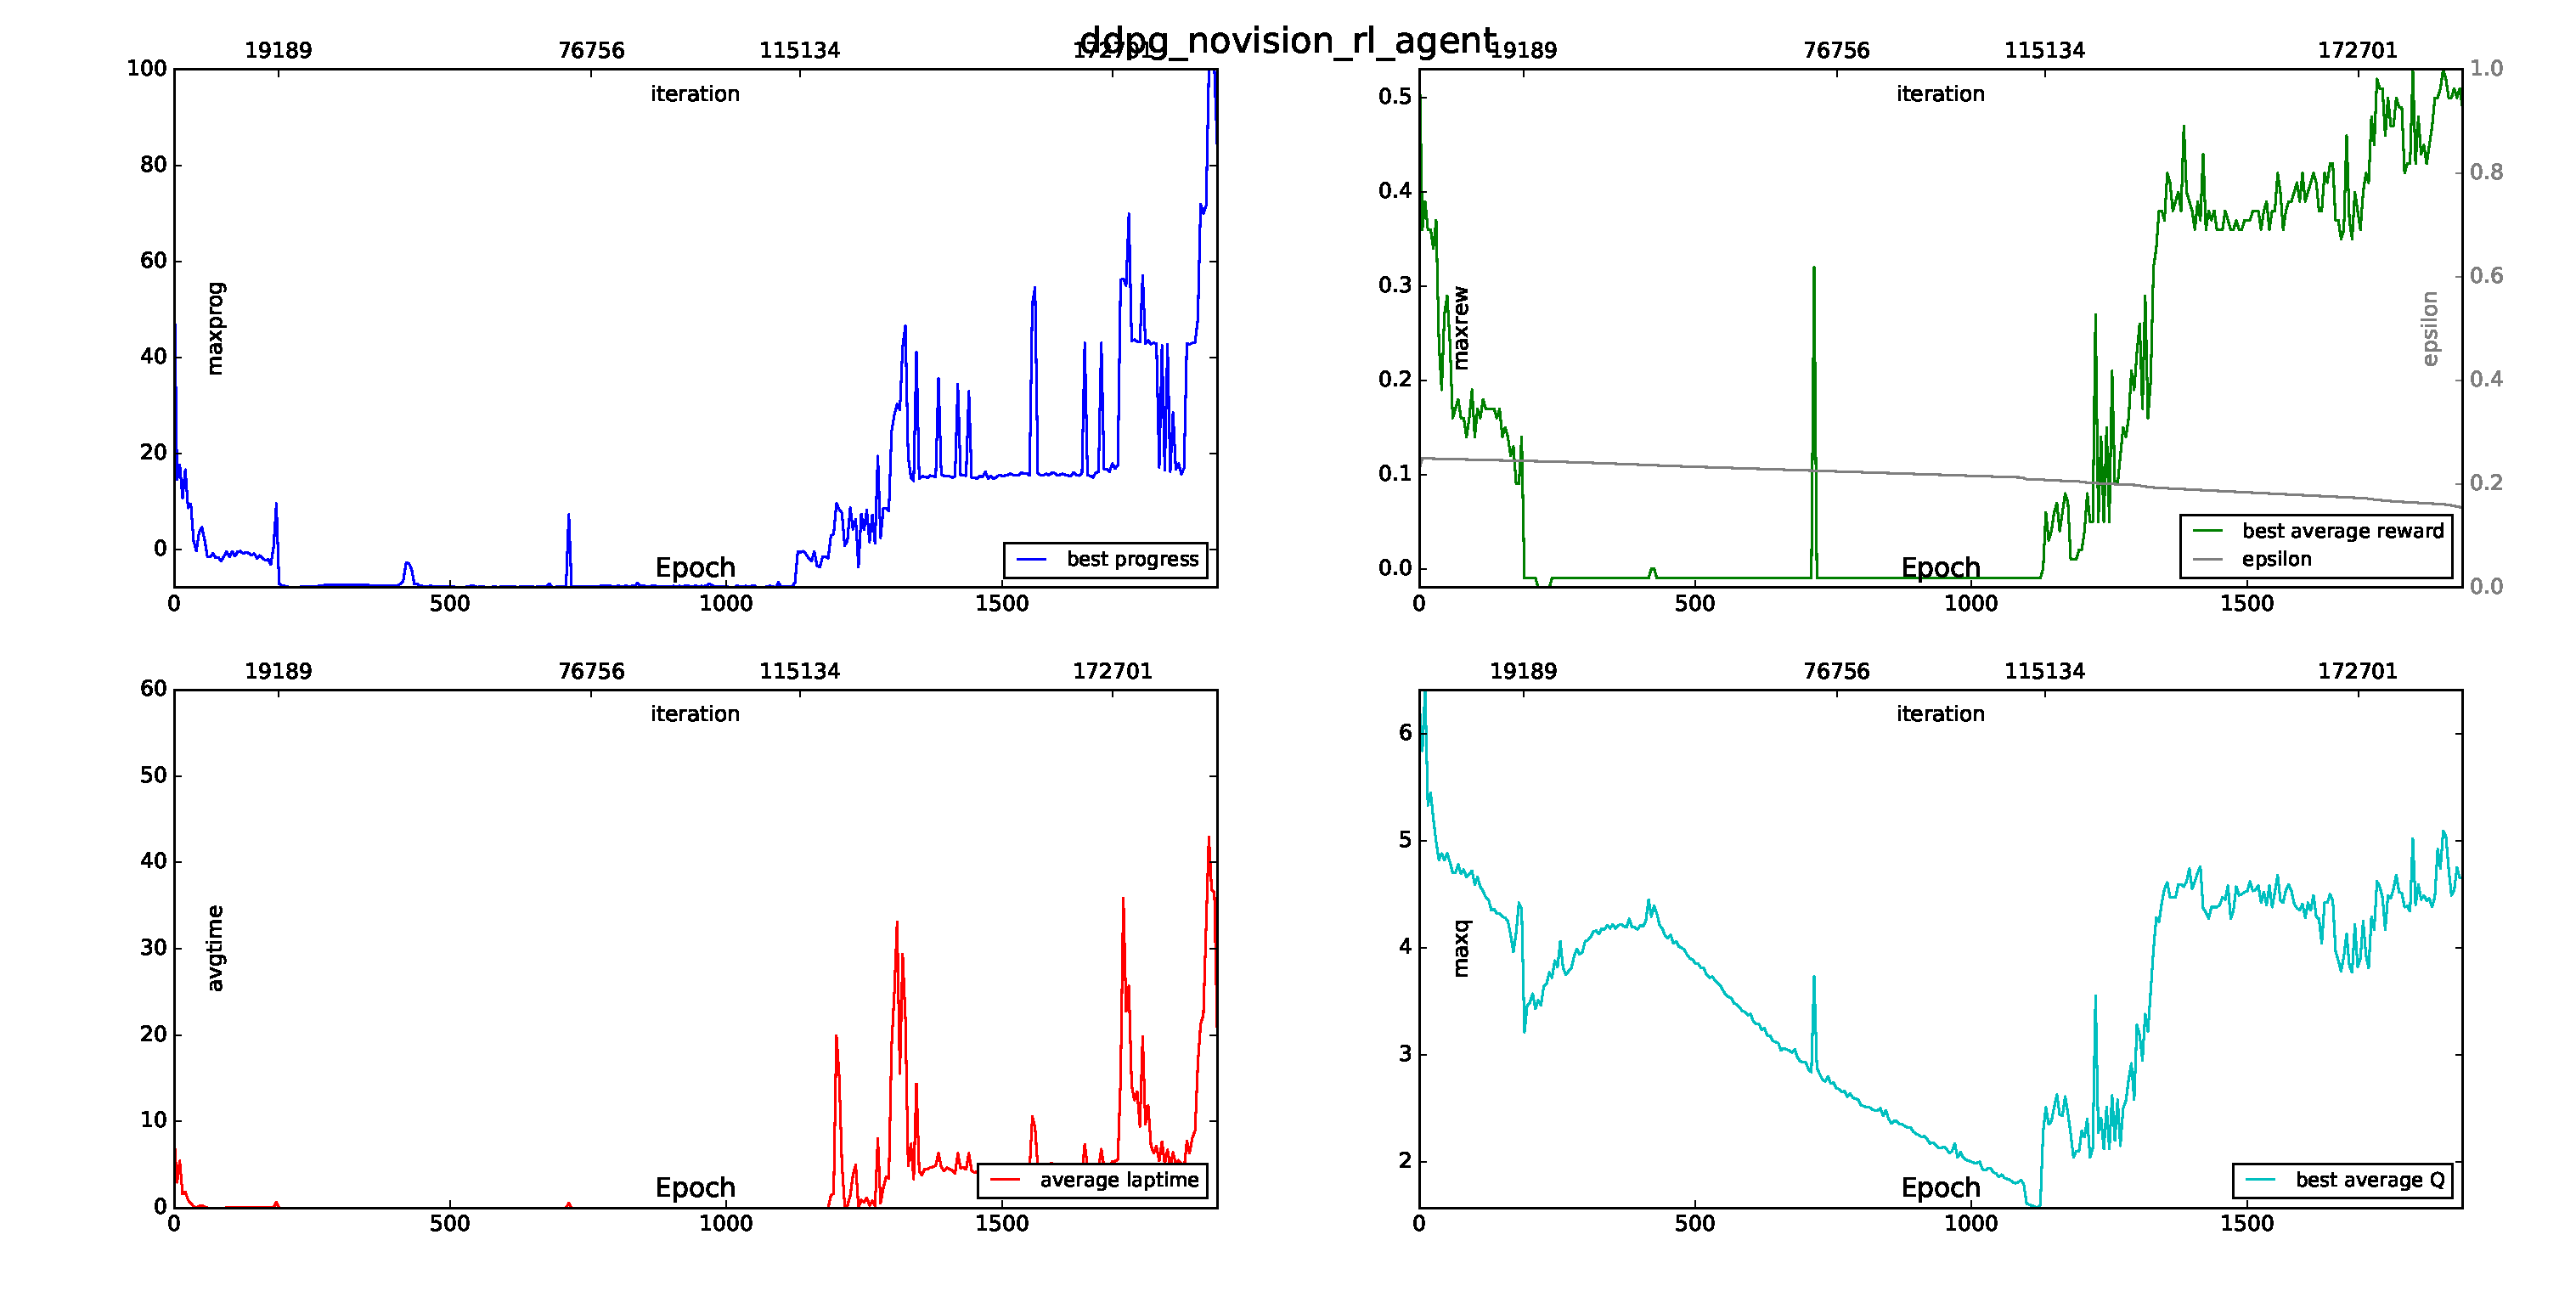
\includegraphics[trim={2.2cm 0cm 1cm 0cm},clip,width=\textwidth]{performance_plots/ddpg_meinward_average5_1900eps_2500pretrainepisodesauf17datasets}}%
	}%
	\centering
	\caption[Exemplary performance of the ddpg\_novison\_rl\_agent after 40000 pretrain steps]{Exemplary performance of the ddpg\_novison\_rl\_agent after 40000 pretraining steps. Plots are smoothed by averaging over 5 episodes.}
	\label{fig:ddpg_incorpPre}
\end{figure}

All in all, this agent completed its first full circuit after around 1900 episodes, more than 500 epochs later than an agent that did not perform pretraining. 

While not printed in this thesis, the plot of a pretrained \term{dqn\_novision\_rl\_agent} showed the same properties than the one described.

Concluding it must be said, that this thesis did not find a successful way to incorporate a pretraining based on manually driven rounds. This can be due to three main reasons: 1) the dataset was to small and must be extended, 2) it is simply not possible to learn from only \textit{good} rounds, or 3) the employed method is not the correct approach. Further resarch must be taken, especially trying to find a better method than the used one.

\section{Reward function}

One of the research questions asked \textit{what a good reward function looks like, that rewards the \textit{correct} behaviour at all times (including braking)}. All agents of the previously mentioned figures used the reward function from section~\ref{sec:reward}. The fact that these agents succeeded is evidence that incorporating this function contributes to successful driving policies. For this section, this method is compared with two other reward functions. 

\begin{figure}[h]
	{%
		\setlength{\fboxsep}{0pt}%
		\setlength{\fboxrule}{1pt}%
		\fbox{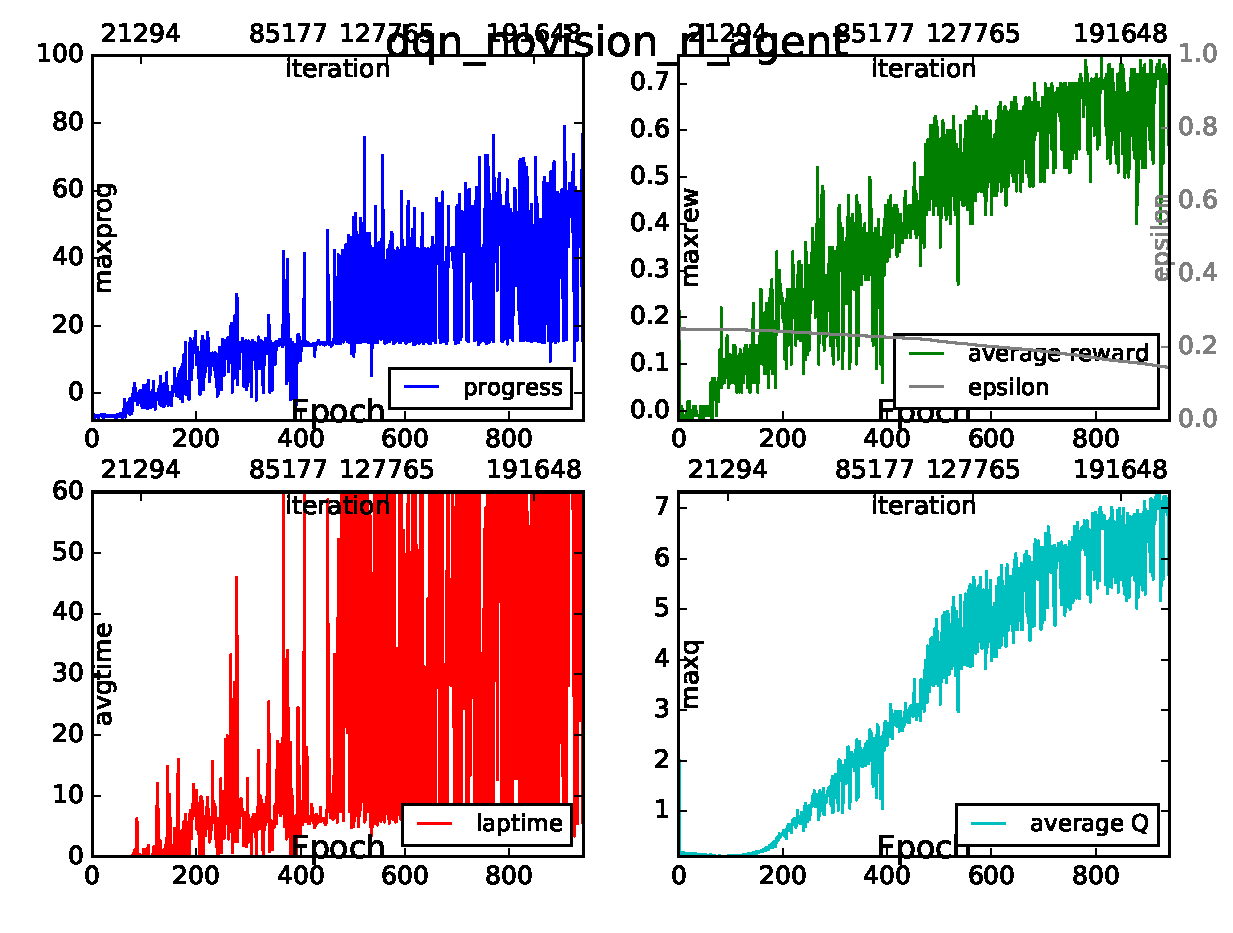
\includegraphics[width=\textwidth]{performance_plots/dqn_rewardinrelationtowalldist_smooth1_900ep}}%
	}%
	\centering
	\caption[Exemplary performance of the dqn\_novison\_rl\_agent with SpeedInRelationToWallDist as only reward.]{Exemplary performance of the dqn\_novison\_rl\_agent with SpeedInRelationToWallDist as only reward. Plots are not smoothed.}
	\label{fig:dqnrewardinrelationtowall}
\end{figure}

In the original DDPG-Paper, the authors used as reward only \textit{the velocity of the car projected along the track direction and a penalty of -1 for collisions.}(quote \cite{lillicrap_continuous_2015}). In the given simulation, this corresponds to the feature \codeobj{SpeedSteer.SpeedInStreetDir}, with the collision punished in \codefunc{handle\_commands}. Figure~\ref{fig:dqnrewardspeedstuff} shows the performance of an agent that uses this reward function. 
As can be seen in the respective plot, this reward does not lead to successful results after $2500$ episodes, whereas the its average reward is almost maximal. As this reward function does not reward braking at all, the agent does not learn so and almost every episode ends with the car skidding at the first turn.


\begin{figure}[h]
	{%
		\setlength{\fboxsep}{0pt}%
		\setlength{\fboxrule}{1pt}%
		\fbox{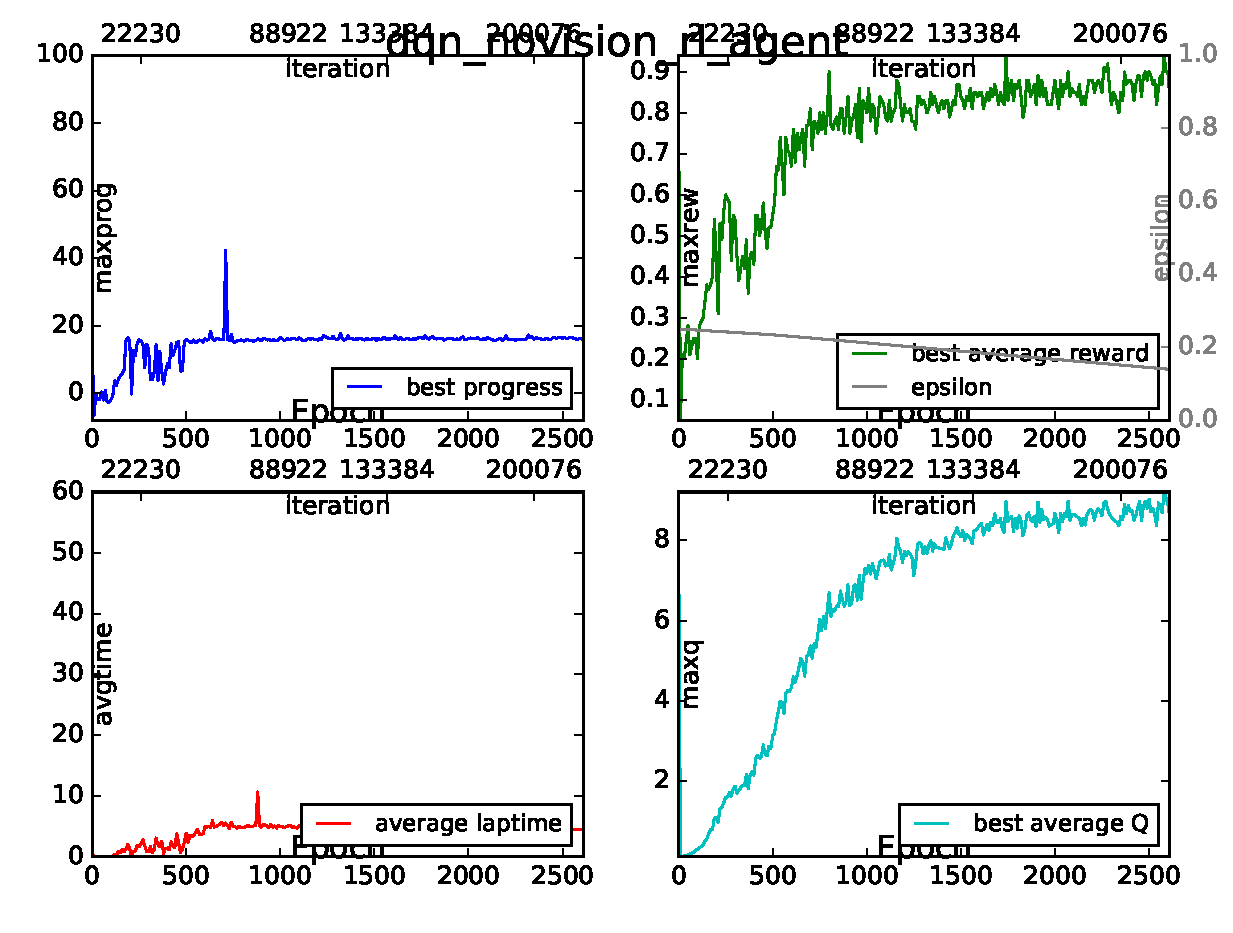
\includegraphics[width=\textwidth]{performance_plots/dqn_rewardspeed_smooth10_2600ep}}%
	}%
	\centering
	\caption[Exemplary performance of the dqn\_novison\_rl\_agent with the reward function from \cite{lillicrap_continuous_2015}]{Exemplary performance of the dqn\_novison\_rl\_agent with the reward function from \cite{lillicrap_continuous_2015}. Plots are smoothed by averaging over 10 episodes.}
	\label{fig:dqnrewardspeedstuff}
\end{figure}


To demonstrate the contributions of the other reward-components, figure~\ref{fig:dqnrewardinrelationtowall} shows the performance of an agent with the other reward-components removed (corresponding to lines 1-4 from algorithm~\ref{alg:speedinrelationto}). While the progress makes it appear that the agent learns a useful policy, the plot of the lap-time shows that almost every episode ended because of the time limitof 60 seconds. As this reward-function does always reward driving fast, it is no reasonable reward-function on its own.